\PassOptionsToPackage{unicode=true}{hyperref} % options for packages loaded elsewhere
\PassOptionsToPackage{hyphens}{url}
%
\documentclass[ignorenonframetext,]{beamer}
\usepackage{pgfpages}
\setbeamertemplate{caption}[numbered]
\setbeamertemplate{caption label separator}{: }
\setbeamercolor{caption name}{fg=normal text.fg}
\beamertemplatenavigationsymbolsempty
% Prevent slide breaks in the middle of a paragraph:
\widowpenalties 1 10000
\raggedbottom
\setbeamertemplate{part page}{
\centering
\begin{beamercolorbox}[sep=16pt,center]{part title}
  \usebeamerfont{part title}\insertpart\par
\end{beamercolorbox}
}
\setbeamertemplate{section page}{
\centering
\begin{beamercolorbox}[sep=12pt,center]{part title}
  \usebeamerfont{section title}\insertsection\par
\end{beamercolorbox}
}
\setbeamertemplate{subsection page}{
\centering
\begin{beamercolorbox}[sep=8pt,center]{part title}
  \usebeamerfont{subsection title}\insertsubsection\par
\end{beamercolorbox}
}
\AtBeginPart{
  \frame{\partpage}
}
\AtBeginSection{
  \ifbibliography
  \else
    \frame{\sectionpage}
  \fi
}
\AtBeginSubsection{
  \frame{\subsectionpage}
}
\usepackage{lmodern}
\usepackage{amssymb,amsmath}
\usepackage{ifxetex,ifluatex}
\usepackage{fixltx2e} % provides \textsubscript
\ifnum 0\ifxetex 1\fi\ifluatex 1\fi=0 % if pdftex
  \usepackage[T1]{fontenc}
  \usepackage[utf8]{inputenc}
  \usepackage{textcomp} % provides euro and other symbols
\else % if luatex or xelatex
  \usepackage{unicode-math}
  \defaultfontfeatures{Ligatures=TeX,Scale=MatchLowercase}
\fi
% use upquote if available, for straight quotes in verbatim environments
\IfFileExists{upquote.sty}{\usepackage{upquote}}{}
% use microtype if available
\IfFileExists{microtype.sty}{%
\usepackage[]{microtype}
\UseMicrotypeSet[protrusion]{basicmath} % disable protrusion for tt fonts
}{}
\IfFileExists{parskip.sty}{%
\usepackage{parskip}
}{% else
\setlength{\parindent}{0pt}
\setlength{\parskip}{6pt plus 2pt minus 1pt}
}
\usepackage{hyperref}
\hypersetup{
            pdftitle={Tema 7 - Intervalos de confianza},
            pdfauthor={Ricardo Alberich, Juan Gabriel Gomila y Arnau Mir},
            pdfborder={0 0 0},
            breaklinks=true}
\urlstyle{same}  % don't use monospace font for urls
\newif\ifbibliography
\usepackage{color}
\usepackage{fancyvrb}
\newcommand{\VerbBar}{|}
\newcommand{\VERB}{\Verb[commandchars=\\\{\}]}
\DefineVerbatimEnvironment{Highlighting}{Verbatim}{commandchars=\\\{\}}
% Add ',fontsize=\small' for more characters per line
\usepackage{framed}
\definecolor{shadecolor}{RGB}{248,248,248}
\newenvironment{Shaded}{\begin{snugshade}}{\end{snugshade}}
\newcommand{\AlertTok}[1]{\textcolor[rgb]{0.94,0.16,0.16}{#1}}
\newcommand{\AnnotationTok}[1]{\textcolor[rgb]{0.56,0.35,0.01}{\textbf{\textit{#1}}}}
\newcommand{\AttributeTok}[1]{\textcolor[rgb]{0.77,0.63,0.00}{#1}}
\newcommand{\BaseNTok}[1]{\textcolor[rgb]{0.00,0.00,0.81}{#1}}
\newcommand{\BuiltInTok}[1]{#1}
\newcommand{\CharTok}[1]{\textcolor[rgb]{0.31,0.60,0.02}{#1}}
\newcommand{\CommentTok}[1]{\textcolor[rgb]{0.56,0.35,0.01}{\textit{#1}}}
\newcommand{\CommentVarTok}[1]{\textcolor[rgb]{0.56,0.35,0.01}{\textbf{\textit{#1}}}}
\newcommand{\ConstantTok}[1]{\textcolor[rgb]{0.00,0.00,0.00}{#1}}
\newcommand{\ControlFlowTok}[1]{\textcolor[rgb]{0.13,0.29,0.53}{\textbf{#1}}}
\newcommand{\DataTypeTok}[1]{\textcolor[rgb]{0.13,0.29,0.53}{#1}}
\newcommand{\DecValTok}[1]{\textcolor[rgb]{0.00,0.00,0.81}{#1}}
\newcommand{\DocumentationTok}[1]{\textcolor[rgb]{0.56,0.35,0.01}{\textbf{\textit{#1}}}}
\newcommand{\ErrorTok}[1]{\textcolor[rgb]{0.64,0.00,0.00}{\textbf{#1}}}
\newcommand{\ExtensionTok}[1]{#1}
\newcommand{\FloatTok}[1]{\textcolor[rgb]{0.00,0.00,0.81}{#1}}
\newcommand{\FunctionTok}[1]{\textcolor[rgb]{0.00,0.00,0.00}{#1}}
\newcommand{\ImportTok}[1]{#1}
\newcommand{\InformationTok}[1]{\textcolor[rgb]{0.56,0.35,0.01}{\textbf{\textit{#1}}}}
\newcommand{\KeywordTok}[1]{\textcolor[rgb]{0.13,0.29,0.53}{\textbf{#1}}}
\newcommand{\NormalTok}[1]{#1}
\newcommand{\OperatorTok}[1]{\textcolor[rgb]{0.81,0.36,0.00}{\textbf{#1}}}
\newcommand{\OtherTok}[1]{\textcolor[rgb]{0.56,0.35,0.01}{#1}}
\newcommand{\PreprocessorTok}[1]{\textcolor[rgb]{0.56,0.35,0.01}{\textit{#1}}}
\newcommand{\RegionMarkerTok}[1]{#1}
\newcommand{\SpecialCharTok}[1]{\textcolor[rgb]{0.00,0.00,0.00}{#1}}
\newcommand{\SpecialStringTok}[1]{\textcolor[rgb]{0.31,0.60,0.02}{#1}}
\newcommand{\StringTok}[1]{\textcolor[rgb]{0.31,0.60,0.02}{#1}}
\newcommand{\VariableTok}[1]{\textcolor[rgb]{0.00,0.00,0.00}{#1}}
\newcommand{\VerbatimStringTok}[1]{\textcolor[rgb]{0.31,0.60,0.02}{#1}}
\newcommand{\WarningTok}[1]{\textcolor[rgb]{0.56,0.35,0.01}{\textbf{\textit{#1}}}}
\usepackage{graphicx,grffile}
\makeatletter
\def\maxwidth{\ifdim\Gin@nat@width>\linewidth\linewidth\else\Gin@nat@width\fi}
\def\maxheight{\ifdim\Gin@nat@height>\textheight\textheight\else\Gin@nat@height\fi}
\makeatother
% Scale images if necessary, so that they will not overflow the page
% margins by default, and it is still possible to overwrite the defaults
% using explicit options in \includegraphics[width, height, ...]{}
\setkeys{Gin}{width=\maxwidth,height=\maxheight,keepaspectratio}
\setlength{\emergencystretch}{3em}  % prevent overfull lines
\providecommand{\tightlist}{%
  \setlength{\itemsep}{0pt}\setlength{\parskip}{0pt}}
\setcounter{secnumdepth}{0}

% set default figure placement to htbp
\makeatletter
\def\fps@figure{htbp}
\makeatother

\usepackage{tikz}

\title{Tema 7 - Intervalos de confianza}
\author{Ricardo Alberich, Juan Gabriel Gomila y Arnau Mir}
\date{null}

\begin{document}
\frame{\titlepage}

\hypertarget{definiciones-basicas}{%
\section{Definiciones básicas}\label{definiciones-basicas}}

\begin{frame}{Estimación por intervalos}
\protect\hypertarget{estimacion-por-intervalos}{}

Una estimación por intervalos de un parámetro poblacional es una regla
para calcular, a partir de una muestra, un intervalo en el que, con una
cierta probabilidad (nivel de confianza), se encuentra el valor
verdadero del parámetro.

Estas reglas definirán, a su vez, estimadores.

\end{frame}

\begin{frame}{Estimación por intervalos. Ejemplos}
\protect\hypertarget{estimacion-por-intervalos.-ejemplos}{}

Hemos escogido al azar 50 estudiantes de grado de la UIB, hemos
calculada sus notas medias de las asignaturas del primer semestre, y la
media de estas medias ha sido un 6.3, con una varianza muestral de 1.8.

Determinar un intervalo del que podamos afirmar con probabilidad 95\%
que contiene la media real de las notas medias de los estudiantes de
grado de la UIB este primer semestre.

En un experimento en el que se ha medido la tasa oficial de alcoholemia
en sangre a 40 varones (sobrios) después de tomar 3 cañas de cerveza de
330 ml. La media y la desviación típica de esta tasa han sido \[
\overline{x}=0.7,\quad \widetilde{s}=0.1.
\] Determinar un intervalo que podamos afirmar con probabilidad 95\% que
contiene la tasa de alcoholemia media en sangre de una varón después de
beber 3 cañas de cerveza de 330 ml.

\end{frame}

\begin{frame}{Definición de intervalo de confianza}
\protect\hypertarget{definicion-de-intervalo-de-confianza}{}

Intervalo de confianza. Dado un parámetro \(\theta\), el intervalo
\(]A,B[\) es un intervalo de confianza del \((1-\alpha)\cdot 100\)\%
para al parámetro \(\theta\) cuando \[
P(A<\theta<B)=1-\alpha.
\] El valor \((1-\alpha)\cdot 100\)\% (o contiene solo el \(1-\alpha\))
recibe el nombre de nivel de confianza.

El valor \(\alpha\) recibe el nombre de nivel de significación.

\end{frame}

\begin{frame}{Definición de intervalo de confianza}
\protect\hypertarget{definicion-de-intervalo-de-confianza-1}{}

Por defecto, buscaremos intervalos bilaterales tales que la \textbf{cola
de probabilidad sobrante} \(\alpha\) se reparta por igual a cada lado
del intervalo: \[
P(\theta<A)=P(\theta>B)=\frac{\alpha}{2}
\]

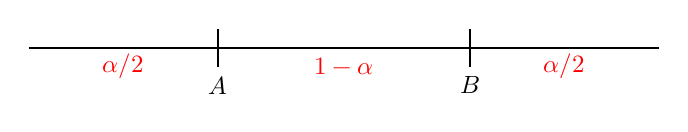
\begin{tikzpicture}[thick,scale=0.8]%[>=stealth]%,yscale=0.5,xscale=0.7]
\draw (0,0)--(10,0);
\draw (3,0.3)--(3,-0.3);
\draw (7,0.3)--(7,-0.3);
\draw(3,-0.6) node {\small $A$}; 
\draw (7,-0.6) node {\small $B$}; 
\draw[red] (8.5,-0.3) node {\small $\alpha/2$}; 
\draw[red] (1.5,-0.3) node {\small $\alpha/2$}; 
\draw[red] (5,-0.3) node {\small $1-\alpha$}; 
\end{tikzpicture}

\end{frame}

\begin{frame}{Intervalos de confianza}
\protect\hypertarget{intervalos-de-confianza}{}

\begin{itemize}
\tightlist
\item
  Un \textbf{intervalo de confianza del \(q\times 100\%\)}
  (\(0\leq q\leq 1\)) para un parámetro poblacional es un intervalo
  obtenido a partir de una muestra que garantiza (si se cumplen una
  serie de condiciones sobre la distribución de la variable aleatoria
  poblacional que en cada caso dependen del parámetro y de la fórmula)
  que el \(q\times 100\%\) de las veces que la aplicásemos a una muestra
  aleatoria simple de la misma población, el intervalo resultante
  contendría el parámetro poblacional.
\end{itemize}

\end{frame}

\begin{frame}{Intervalo de confianza para la media basado en la t de
Student}
\protect\hypertarget{intervalo-de-confianza-para-la-media-basado-en-la-t-de-student}{}

\begin{itemize}
\item
  Queremos estimar a partir de una m.a.s. la media \(\mu\) de una
  población que sigue una distribución normal o tomando la muestra
  grande (\(n\geq 40\)).
\item
  Sean \(\overline{X}\), \(\widetilde{S}_{X}\), y \(n\), la media
  muestral, la desviación típica muestral y el tamaño de la muestra,
  respectivamente.
\item
  Un intervalo de confianza del \(q\times 100\%\) para \(\mu\) es \[
  \overline{X}\pm t_{n-1,(1+q)/2} \cdot \frac{\widetilde{S}_{X}}{\sqrt{n}},
  \] donde \(t_{n-1,(1+q)/2}\) es el cuantil de orden \((1+q)/2\) de una
  variable aleatoria con distribución t de Student con \(n-1\) grados de
  libertad.
\end{itemize}

\end{frame}

\begin{frame}[fragile]{Intervalo de confianza para la media basado en la
t de Student en \texttt{R}}
\protect\hypertarget{intervalo-de-confianza-para-la-media-basado-en-la-t-de-student-en-r}{}

\begin{itemize}
\item
\begin{verbatim}
t.test(X,conf.level=...)$conf.int
\end{verbatim}

  donde \texttt{conf.level} es el nivel de confianza \(q\) en tanto por
  uno. Valor por defecto: \(q=0.95\).
\end{itemize}

\end{frame}

\begin{frame}[fragile]{Intervalo de confianza para la media basado en la
t de Student en \texttt{R}}
\protect\hypertarget{intervalo-de-confianza-para-la-media-basado-en-la-t-de-student-en-r-1}{}

Hallemos un intervalo de confianza para la media de la longitud del
pétalo para una muestra de 30 flores de la tabla de datos \textbf{iris}:

\begin{itemize}
\tightlist
\item
  En primer lugar elegimos las flores de la muestra:
\end{itemize}

\begin{Shaded}
\begin{Highlighting}[]
\KeywordTok{set.seed}\NormalTok{(}\DecValTok{1000}\NormalTok{)}
\NormalTok{muestra.iris =}\StringTok{ }\KeywordTok{sample}\NormalTok{(}\DecValTok{1}\OperatorTok{:}\DecValTok{150}\NormalTok{,}\DecValTok{30}\NormalTok{,}\DataTypeTok{replace=}\OtherTok{TRUE}\NormalTok{)}
\end{Highlighting}
\end{Shaded}

A continuación calculamos las longitudes del pétalo de las flores de
nuestra muestra:

\begin{Shaded}
\begin{Highlighting}[]
\NormalTok{long.pétalo.muestra =}\StringTok{ }\NormalTok{iris[muestra.iris,]}\OperatorTok{$}\NormalTok{Petal.Length}
\end{Highlighting}
\end{Shaded}

\end{frame}

\begin{frame}[fragile]{Intervalo de confianza para la media basado en la
t de Student en \texttt{R}}
\protect\hypertarget{intervalo-de-confianza-para-la-media-basado-en-la-t-de-student-en-r-2}{}

Un intervalo de confianza al 95\% de confianza para las longitudes del
pétalo sería:

\begin{Shaded}
\begin{Highlighting}[]
\KeywordTok{t.test}\NormalTok{(long.pétalo.muestra,}\DataTypeTok{conf.level=}\FloatTok{0.95}\NormalTok{)}\OperatorTok{$}\NormalTok{conf.int}
\end{Highlighting}
\end{Shaded}

\begin{verbatim}
## [1] 2.986537 4.106796
## attr(,"conf.level")
## [1] 0.95
\end{verbatim}

\end{frame}

\begin{frame}[fragile]{Intervalo de confianza para la media basado en la
t de Student en \texttt{R}}
\protect\hypertarget{intervalo-de-confianza-para-la-media-basado-en-la-t-de-student-en-r-3}{}

Vamos a comprobar con un experimento qué papel juega la ``confianza'' en
los intervalos de confianza.

Vamos a generar al azar una Población de 10000000 (\(10^7\))
``individuos'' con distribución normal estándard. Vamos a tomar 200
muestras aleatorias simples de tamaño 50 de esta población y
calcularemos el intervalo de confianza para la media poblacional usando
dicha fórmula.

Finalmente, contaremos cuántos de estos intervalos de confianza
contienen la media de la población. Fijaremos la semilla de aleatoriedad
para que el experimento sea reproducible y podáis comprobar que no
hacemos trampa.

En primer lugar, generamos la población de valores:

\begin{Shaded}
\begin{Highlighting}[]
\KeywordTok{set.seed}\NormalTok{(}\DecValTok{2020}\NormalTok{)}
\NormalTok{valores.población=}\KeywordTok{rnorm}\NormalTok{(}\DecValTok{10}\OperatorTok{^}\DecValTok{7}\NormalTok{)}
\end{Highlighting}
\end{Shaded}

Seguidamente, hallamos la media poblacional:

\begin{Shaded}
\begin{Highlighting}[]
\NormalTok{mu=}\KeywordTok{mean}\NormalTok{(valores.población)}
\end{Highlighting}
\end{Shaded}

\end{frame}

\begin{frame}[fragile]{Intervalo de confianza para la media basado en la
t de Student en \texttt{R}}
\protect\hypertarget{intervalo-de-confianza-para-la-media-basado-en-la-t-de-student-en-r-4}{}

Para hallar 200 muestras, usaremos la función \texttt{replicate} de
\texttt{R} que nos permite ejecutar una misma función las veces que le
indiquemos:

\begin{Shaded}
\begin{Highlighting}[]
\NormalTok{muestras=}\KeywordTok{replicate}\NormalTok{(}\DecValTok{200}\NormalTok{, }\KeywordTok{sample}\NormalTok{(valores.población,}\DecValTok{50}\NormalTok{,}\DataTypeTok{replace=}\OtherTok{TRUE}\NormalTok{))}
\end{Highlighting}
\end{Shaded}

De esta forma \texttt{muestras} es una matriz de 50 filas y 200 columnas
donde cada fila representa una muestra.

A continuación, Vamos a aplicar a cada una de estas muestras la función
\texttt{t.test} para calcular un intervalo de confianza del 95\% y luego
contaremos los aciertos, es decir, cuántos de ellos contienen la media
poblacional.

Primero definimos la función \texttt{IC.t} que nos da el intervalo de
confianza para la media dada una muestra \texttt{X}:

\begin{Shaded}
\begin{Highlighting}[]
\NormalTok{IC.t=}\StringTok{ }\ControlFlowTok{function}\NormalTok{(X)\{}\KeywordTok{t.test}\NormalTok{(X)}\OperatorTok{$}\NormalTok{conf.int\}}
\end{Highlighting}
\end{Shaded}

\end{frame}

\begin{frame}[fragile]{Intervalo de confianza para la media basado en la
t de Student en \texttt{R}}
\protect\hypertarget{intervalo-de-confianza-para-la-media-basado-en-la-t-de-student-en-r-5}{}

En segundo lugar, calculamos los 200 intervalos de confianza para
nuestras 200 muestras usando la función \texttt{apply} de \texttt{R}:

\begin{Shaded}
\begin{Highlighting}[]
\NormalTok{ICs=}\StringTok{ }\KeywordTok{apply}\NormalTok{(muestras,}\DataTypeTok{FUN=}\NormalTok{IC.t,}\DataTypeTok{MARGIN=}\DecValTok{2}\NormalTok{)}
\end{Highlighting}
\end{Shaded}

En tercer lugar, miramos cuántos de los intervalos anteriores contienen
la media poblacional \texttt{mu}:

\begin{Shaded}
\begin{Highlighting}[]
\NormalTok{Aciertos=}\KeywordTok{length}\NormalTok{(}\KeywordTok{which}\NormalTok{((mu}\OperatorTok{>=}\NormalTok{ICs[}\DecValTok{1}\NormalTok{,]) }\OperatorTok{&}\StringTok{ }\NormalTok{(mu}\OperatorTok{<=}\NormalTok{ICs[}\DecValTok{2}\NormalTok{,])))}
\NormalTok{Aciertos}
\end{Highlighting}
\end{Shaded}

\begin{verbatim}
## [1] 195
\end{verbatim}

Hemos acertado 195 veces, o sea, el 97.5\% de las veces. Es una buena
aproximación del valor 95\%, que era el esperado.

\end{frame}

\begin{frame}[fragile]{Intervalo de confianza para la media basado en la
t de Student en \texttt{R}}
\protect\hypertarget{intervalo-de-confianza-para-la-media-basado-en-la-t-de-student-en-r-6}{}

Para visualizar mejor los aciertos, vamos a dibujar los intervalos
apilados en un gráfico, donde aparecerán en azul claro los que aciertan
y en rojo los que no aciertan.

\begin{Shaded}
\begin{Highlighting}[]
\KeywordTok{plot}\NormalTok{(}\DecValTok{1}\NormalTok{,}\DataTypeTok{type=}\StringTok{"n"}\NormalTok{,}\DataTypeTok{xlim=}\KeywordTok{c}\NormalTok{(}\OperatorTok{-}\FloatTok{0.8}\NormalTok{,}\FloatTok{0.8}\NormalTok{),}\DataTypeTok{ylim=}\KeywordTok{c}\NormalTok{(}\DecValTok{0}\NormalTok{,}\DecValTok{200}\NormalTok{),}\DataTypeTok{xlab=}\StringTok{"Valores"}\NormalTok{,}\DataTypeTok{ylab=}\StringTok{"Repeticiones"}\NormalTok{,}\DataTypeTok{main=}\StringTok{""}\NormalTok{)}
\NormalTok{seg.int=}\ControlFlowTok{function}\NormalTok{(i)\{}
\NormalTok{  color=}\StringTok{"light blue"}\NormalTok{;}
  \ControlFlowTok{if}\NormalTok{((mu}\OperatorTok{<}\NormalTok{ICs[}\DecValTok{1}\NormalTok{,i]) }\OperatorTok{|}\StringTok{ }\NormalTok{(mu}\OperatorTok{>}\NormalTok{ICs[}\DecValTok{2}\NormalTok{,i]))\{color =}\StringTok{ "red"}\NormalTok{\}}
  \KeywordTok{segments}\NormalTok{(ICs[}\DecValTok{1}\NormalTok{,i],i,ICs[}\DecValTok{2}\NormalTok{,i],i,}\DataTypeTok{col=}\NormalTok{color,}\DataTypeTok{lwd=}\DecValTok{2}\NormalTok{)}
\NormalTok{  \}}
\KeywordTok{sapply}\NormalTok{(}\DecValTok{1}\OperatorTok{:}\DecValTok{200}\NormalTok{,}\DataTypeTok{FUN=}\NormalTok{seg.int);}
\KeywordTok{abline}\NormalTok{(}\DataTypeTok{v=}\NormalTok{mu,}\DataTypeTok{lwd=}\DecValTok{2}\NormalTok{)}
\end{Highlighting}
\end{Shaded}

\end{frame}

\begin{frame}{Intervalo de confianza para la media basado en la t de
Student en \texttt{R}}
\protect\hypertarget{intervalo-de-confianza-para-la-media-basado-en-la-t-de-student-en-r-7}{}

\includegraphics{Tema-7---IC_files/figure-beamer/unnamed-chunk-11-1.pdf}

\end{frame}

\begin{frame}{Intervalos de confianza para la proporción poblacional.
Método de Clopper-Pearson.}
\protect\hypertarget{intervalos-de-confianza-para-la-proporcion-poblacional.-metodo-de-clopper-pearson.}{}

\begin{itemize}
\item
  Supongamos que tenemos una población distribuida según una variable
  Bernoulli y queremos estimar su probabilidad de éxito (o
  \textbf{proporción poblacional}) \(p\).
\item
  Tomamos una muestra aleatoria simple de tamaño \(n\) y número de
  éxitos \(x\), y, por lo tanto, de \textbf{proporción muestral} de
  éxitos \(\widehat{p}_X=x/n\).
\item
  El \textbf{Método ``exacto'' de Clopper-Pearson} consiste en hallar
  los valores \(p_0\) y \(p_1\) tales que \[
  \begin{array}{ll}
  \sum\limits_{k=x}^n\binom{n}{k}p_0^k(1-p_0)^{n-k} & =(1-q)/2,\\
  \sum\limits_{k=0}^x\binom{n}{k}p_1^k(1-p_1)^{n-k} & =(1-q)/2.
  \end{array}
  \]
\end{itemize}

\end{frame}

\begin{frame}[fragile]{Intervalos de confianza para la proporción
poblacional. Método de Clopper-Pearson.}
\protect\hypertarget{intervalos-de-confianza-para-la-proporcion-poblacional.-metodo-de-clopper-pearson.-1}{}

\begin{itemize}
\tightlist
\item
  Para hallar un intervalo de confianza para la proporción poblacional
  en \texttt{R} según el método de Clopper-Pearson, hay que usar la
  función \texttt{binom.exact} del paquete \textbf{epitools}:
\end{itemize}

\begin{Shaded}
\begin{Highlighting}[]
\KeywordTok{binom.exact}\NormalTok{(x,n,conf.level)}
\end{Highlighting}
\end{Shaded}

donde \texttt{x} y \texttt{n} representan, respectivamente, el número de
éxitos y el tamaño de la muestra, y \texttt{conf.level} es \(q\), el
nivel de confianza en tanto por uno.

\end{frame}

\begin{frame}[fragile]{Intervalos de confianza para la proporción
poblacional. Método de Clopper-Pearson.}
\protect\hypertarget{intervalos-de-confianza-para-la-proporcion-poblacional.-metodo-de-clopper-pearson.-2}{}

Hallemos un intervalo de confianza para la proporción de flores con
especie ``setosa'' dada una muestra de 60 flores.

Sabemos que la proporción real \(p\) en este caso vale
\(p=\frac{50}{150}=\frac{1}{3}=0.333\).

Primero hallamos la muestra de las 60 flores:

\begin{Shaded}
\begin{Highlighting}[]
\KeywordTok{set.seed}\NormalTok{(}\DecValTok{1000}\NormalTok{)}
\NormalTok{flores.elegidas =}\StringTok{ }\KeywordTok{sample}\NormalTok{(}\DecValTok{1}\OperatorTok{:}\DecValTok{150}\NormalTok{,}\DecValTok{60}\NormalTok{,}\DataTypeTok{replace=}\OtherTok{TRUE}\NormalTok{)}
\end{Highlighting}
\end{Shaded}

\end{frame}

\begin{frame}[fragile]{Intervalos de confianza para la proporción
poblacional. Método de Clopper-Pearson.}
\protect\hypertarget{intervalos-de-confianza-para-la-proporcion-poblacional.-metodo-de-clopper-pearson.-3}{}

Las flores elegidas son: (sólo mostramos las 10 primeras)

\begin{Shaded}
\begin{Highlighting}[]
\NormalTok{muestra.flores.prop =}\StringTok{ }\NormalTok{iris[flores.elegidas,]}
\KeywordTok{head}\NormalTok{(muestra.flores.prop,}\DecValTok{10}\NormalTok{)}
\end{Highlighting}
\end{Shaded}

\begin{verbatim}
##     Sepal.Length Sepal.Width Petal.Length Petal.Width    Species
## 68           5.8         2.7          4.1         1.0 versicolor
## 43           4.4         3.2          1.3         0.2     setosa
## 51           7.0         3.2          4.7         1.4 versicolor
## 88           6.3         2.3          4.4         1.3 versicolor
## 29           5.2         3.4          1.4         0.2     setosa
## 99           5.1         2.5          3.0         1.1 versicolor
## 61           5.0         2.0          3.5         1.0 versicolor
## 146          6.7         3.0          5.2         2.3  virginica
## 150          5.9         3.0          5.1         1.8  virginica
## 102          5.8         2.7          5.1         1.9  virginica
\end{verbatim}

\end{frame}

\begin{frame}[fragile]{Intervalos de confianza para la proporción
poblacional. Método de Clopper-Pearson.}
\protect\hypertarget{intervalos-de-confianza-para-la-proporcion-poblacional.-metodo-de-clopper-pearson.-4}{}

El número de flores de especie setosa será:

\begin{Shaded}
\begin{Highlighting}[]
\NormalTok{(número.}\DataTypeTok{flores.setosa=}\KeywordTok{table}\NormalTok{(muestra.flores.prop}\OperatorTok{$}\NormalTok{Species}\OperatorTok{==}\StringTok{"setosa"}\NormalTok{)[}\DecValTok{2}\NormalTok{])}
\end{Highlighting}
\end{Shaded}

\begin{verbatim}
## TRUE 
##   21
\end{verbatim}

El intervalo de confianza para la proproción poblacional de flores de
especie setosa al 95\% de confianza será:

\begin{Shaded}
\begin{Highlighting}[]
\KeywordTok{library}\NormalTok{(epitools)}
\KeywordTok{binom.exact}\NormalTok{(número.flores.setosa,}\DecValTok{60}\NormalTok{,}\DataTypeTok{conf.level=}\FloatTok{0.95}\NormalTok{)}
\end{Highlighting}
\end{Shaded}

\begin{verbatim}
##       x  n proportion     lower    upper conf.level
## TRUE 21 60       0.35 0.2313264 0.484028       0.95
\end{verbatim}

\end{frame}

\begin{frame}{Intervalos de confianza para la proporción poblacional.
Método de Clopper-Pearson.}
\protect\hypertarget{intervalos-de-confianza-para-la-proporcion-poblacional.-metodo-de-clopper-pearson.-5}{}

Según el método de Clopper-Pearson, con un 95\% de confianza podemos
decir que en la tabla de datos \textbf{iris} hay entre un 23.13\% y
48.4\% de flores de especie ``setosa''.

\end{frame}

\begin{frame}{Intervalos de confianza para la proporción poblacional.
Método de Wilson.}
\protect\hypertarget{intervalos-de-confianza-para-la-proporcion-poblacional.-metodo-de-wilson.}{}

Supongamos ahora que el tamaño \(n\) de la muestra aleatoria simple es
grande (\(n\geq 40\)). Podemos usar el \textbf{Método de Wilson}, basado
en el \emph{Teorema Central del Límite}: \[
\frac{\widehat{p}_{X}+\frac{z_{(1+q)/2}^2}{2n}\pm z_{(1+q)/2}\sqrt{\frac{\widehat{p}_{X}(1-\widehat{p}_{X})}{n}+\frac{z_{(1+q)/2}^2}{4n^2}}}{1+\frac{z_{(1+q)/2}^2}{n}},
\] donde \(z_{(1+q)/2}\) es el cuantil de orden \((1+q)/2\) de una
variable aleatoria normal estándar.

\end{frame}

\begin{frame}[fragile]{Intervalos de confianza para la proporción
poblacional. Método de Wilson.}
\protect\hypertarget{intervalos-de-confianza-para-la-proporcion-poblacional.-metodo-de-wilson.-1}{}

Para hallar un intervalo de confianza para la proporción poblacional en
\texttt{R} según el método de Wilson, hay que usar la función
\texttt{binom.wilson} del mismo paquete \textbf{epitools}:

\begin{Shaded}
\begin{Highlighting}[]
\KeywordTok{binom.wilson}\NormalTok{(x,n,conf.level)}
\end{Highlighting}
\end{Shaded}

\end{frame}

\begin{frame}[fragile]{Intervalos de confianza para la proporción
poblacional. Método de Wilson.}
\protect\hypertarget{intervalos-de-confianza-para-la-proporcion-poblacional.-metodo-de-wilson.-2}{}

Usando el ejemplo anterior, hallemos un intervalo de confianza para la
proporción de flores de especie ``setosa'' según el método de Wilson al
95\% de confianza:

\begin{Shaded}
\begin{Highlighting}[]
\KeywordTok{binom.wilson}\NormalTok{(número.flores.setosa,}\DecValTok{60}\NormalTok{,}\DataTypeTok{conf.level=}\FloatTok{0.95}\NormalTok{)}
\end{Highlighting}
\end{Shaded}

\begin{verbatim}
##       x  n proportion     lower     upper conf.level
## TRUE 21 60       0.35 0.2416777 0.4763738       0.95
\end{verbatim}

Según el método de Wilson, con un 95\% de confianza podemos decir que en
la tabla de datos \textbf{iris} hay entre un 24.17\% y 47.64\% de flores
de especie ``setosa''.

\end{frame}

\begin{frame}{Intervalos de confianza para la proporción poblacional.
Fórmula de Laplace.}
\protect\hypertarget{intervalos-de-confianza-para-la-proporcion-poblacional.-formula-de-laplace.}{}

\begin{itemize}
\item
  Supongamos que la muestra aleatoria simple es considerablemente más
  grande que la usada en el método de \textbf{Wilson} y que, además, la
  proporción muestral de éxitos \(\widehat{p}_{X}\) está alejada de 0 y
  de 1.
\item
  O sea, \(n\geq 100\) y que \(n\widehat{p}_{X}\geq 10\) y
  \(n(1-\widehat{p}_{X})\geq 10\).
\item
  En este caso, podemos usar la fórmula de \textbf{Laplace}: \[
  \widehat{p}_{X}\pm z_{(1+q)/2}\sqrt{\frac{\widehat{p}_{X}
  (1-\widehat{p}_{X})}{n}}.
  \]
\end{itemize}

\end{frame}

\begin{frame}[fragile]{Intervalos de confianza para la proporción
poblacional. Fórmula de Laplace.}
\protect\hypertarget{intervalos-de-confianza-para-la-proporcion-poblacional.-formula-de-laplace.-1}{}

Para hallar un intervalo de confianza para la proporción poblacional en
\texttt{R} según la fórmula de Laplace, hay que usar la función
\texttt{binom.approx} del mismo paquete \textbf{epitools}:

\begin{Shaded}
\begin{Highlighting}[]
\KeywordTok{binom.approx}\NormalTok{(x,n,conf.level)}
\end{Highlighting}
\end{Shaded}

\end{frame}

\begin{frame}[fragile]{Intervalos de confianza para la proporción
poblacional. Fórmula de Laplace.}
\protect\hypertarget{intervalos-de-confianza-para-la-proporcion-poblacional.-formula-de-laplace.-2}{}

Usando el ejemplo anterior, hallemos un intervalo de confianza para la
proporción de flores de especie ``setosa'' según la fórmula de Laplace
al 95\% de confianza:

\begin{Shaded}
\begin{Highlighting}[]
\KeywordTok{binom.approx}\NormalTok{(número.flores.setosa,}\DecValTok{60}\NormalTok{,}\DataTypeTok{conf.level=}\FloatTok{0.95}\NormalTok{)}
\end{Highlighting}
\end{Shaded}

\begin{verbatim}
##       x  n proportion     lower     upper conf.level
## TRUE 21 60       0.35 0.2293123 0.4706877       0.95
\end{verbatim}

Según la fórmula de Laplace, con un 95\% de confianza podemos decir que
en la tabla de datos \textbf{iris} hay entre un 22.93\% y 47.07\% de
flores de especie ``setosa''.

\end{frame}

\begin{frame}{Intervalo de confianza para la varianza de una población
normal}
\protect\hypertarget{intervalo-de-confianza-para-la-varianza-de-una-poblacion-normal}{}

\begin{itemize}
\item
  Supongamos ahora que queremos estimar la varianza \(\sigma^2\), o la
  desviación típica \(\sigma\), de una población que sigue una
  distribución normal. Tomamos una muestra aleatoria simple de tamaño
  \(n\), y sea \(\tilde{S}_X\) su desviación típica muestral.
\item
  Un intervalo de confianza para la varianza \(\sigma^2\) es: \[
  \left( \frac{(n-1)\widetilde{S}_{X}^2}{\chi_{n-1,(1+q)/2}^2},\
  \frac{(n-1)\widetilde{S}_{X}^2}{\chi_{n-1,(1-q)/2}^2}\right),
  \] donde \(\chi_{n-1,(1-q)/2}^2\) y \(\chi_{n-1,(1+q)/2}^2\) son,
  respectivamente, los cuantiles de orden \((1-q)/2\) y \((1+q)/2\) de
  una variable aleatoria que sigue una distribución \(\chi^2\) con
  \(n-1\) grados de libertad.
\end{itemize}

\end{frame}

\begin{frame}[fragile]{Intervalo de confianza para la varianza de una
población normal}
\protect\hypertarget{intervalo-de-confianza-para-la-varianza-de-una-poblacion-normal-1}{}

\begin{itemize}
\tightlist
\item
  Para hallar un intervalo de confianza para la varianza poblacional en
  \texttt{R} hay que usar la función \texttt{varTest} del paquete
  \textbf{EnvStats}:
\end{itemize}

\begin{Shaded}
\begin{Highlighting}[]
\KeywordTok{varTest}\NormalTok{(X,conf.level)}\OperatorTok{$}\NormalTok{conf.int}
\end{Highlighting}
\end{Shaded}

donde \texttt{X} es el vector que contiene la muestra y
\texttt{conf.level} el nivel de confianza, que por defecto es igual a
0.95.

\end{frame}

\begin{frame}[fragile]{Intervalo de confianza para la varianza de una
población normal}
\protect\hypertarget{intervalo-de-confianza-para-la-varianza-de-una-poblacion-normal-2}{}

Hallemos un intervalo de confianza para la varianza de la amplitud del
sépalo de la tabla de datos \textbf{iris} a partir de la muestra
anterior. Suponemos que dicha variable es normal. Veremos en temas
posteriores cómo se puede comprobar la normalidad de una variable.

Hallemos los valores de la amplitud del sépalo para las flores de
nuestra muestra:

\begin{Shaded}
\begin{Highlighting}[]
\NormalTok{(amplitud.sé}\DataTypeTok{palo.muestra =}\NormalTok{ iris[flores.elegidas,]}\OperatorTok{$}\NormalTok{Sepal.Width)}
\end{Highlighting}
\end{Shaded}

\begin{verbatim}
##  [1] 2.7 3.2 3.2 2.3 3.4 2.5 2.0 3.0 3.0 2.7 3.8 3.4 2.7 3.5 3.5 3.0 2.3
## [18] 3.2 2.0 2.8 2.5 2.3 3.1 3.0 2.3 2.9 3.4 3.1 3.4 2.5 2.6 3.7 2.5 4.4
## [35] 3.0 3.4 2.5 2.5 3.2 3.0 3.3 3.2 3.8 3.6 3.0 3.4 2.8 2.6 2.9 3.1 3.1
## [52] 3.3 3.2 3.2 3.5 3.5 3.0 3.4 3.1 2.3
\end{verbatim}

\end{frame}

\begin{frame}[fragile]{Intervalo de confianza para la varianza de una
población normal}
\protect\hypertarget{intervalo-de-confianza-para-la-varianza-de-una-poblacion-normal-3}{}

Un intervalo de confianza para la varianza de las amplitudes del sépalo
para la tabla de datos \textbf{iris} al 95\% de confianza será:

\begin{Shaded}
\begin{Highlighting}[]
\KeywordTok{library}\NormalTok{(EnvStats)}
\KeywordTok{varTest}\NormalTok{(amplitud.sépalo.muestra,}\DataTypeTok{conf.level=}\FloatTok{0.95}\NormalTok{)}\OperatorTok{$}\NormalTok{conf.int}
\end{Highlighting}
\end{Shaded}

\begin{verbatim}
##       LCL       UCL 
## 0.1625640 0.3365786 
## attr(,"conf.level")
## [1] 0.95
\end{verbatim}

\end{frame}

\begin{frame}{Bootstrap}
\protect\hypertarget{bootstrap}{}

\begin{itemize}
\item
  Cuando no se satisfacen las condiciones teóricas que garantizan que el
  intervalo obtenido contiene el 95\% de las veces el parámetro
  poblacional deseado, podemos recurrir a un método no paramétrico. El
  más utilizado es el \textbf{bootstrap}, que básicamente consiste en:

  \begin{enumerate}
  \item
    \textbf{Remuestrear} la muestra: tomar muchas muestras aleatorias
    simples de la muestra de la que disponemos, cada una de ellas del
    mismo tamaño que la muestra original (pero simples, es decir, con
    reposición).
  \item
    Calcular el estimador sobre cada una de estas submuestras.
  \item
    Organizar los resultados en un vector.
  \item
    Usar este vector para calcular un intervalo de confianza.
  \end{enumerate}
\end{itemize}

\end{frame}

\begin{frame}{Bootstrap: método de los percentiles}
\protect\hypertarget{bootstrap-metodo-de-los-percentiles}{}

\begin{itemize}
\tightlist
\item
  La manera más sencilla de llevar a cabo el cálculo final del intervalo
  de confianza es el llamado \textbf{método de los percentiles} , en el
  que se toman como extremos del intervalo de confianza del
  \(q\times 100%\) los cuantiles de orden \(\frac{1−q}{2}\) y
  \(\frac{1+q}{2}\) del vector de estimadores.
\end{itemize}

\end{frame}

\begin{frame}[fragile]{Bootstrap: método de los percentiles}
\protect\hypertarget{bootstrap-metodo-de-los-percentiles-1}{}

Como aplicación del \textbf{método de los percentiles} hallemos un
intervalo de confianza para la varianza de la longitud del pétalo de la
tabla de datos \textbf{iris}.

No podemos usar la fórmula vista anteriormente ya que la variable
considerada no puede considerarse normal.

Tomaremos la muestra de la tabla de datos \textbf{iris} que hemos
calculado anteriormente en la sección de intervalo de confianza para
proporciones.

Usaremos la función \texttt{replicate} de \texttt{R} para calcular las
varianzas de 1000 muestras ``remuestradas'' de nuestra muestra original:

\begin{Shaded}
\begin{Highlighting}[]
\KeywordTok{set.seed}\NormalTok{(}\DecValTok{42}\NormalTok{)}
\NormalTok{X=}\KeywordTok{replicate}\NormalTok{(}\DecValTok{1000}\NormalTok{, }\KeywordTok{var}\NormalTok{(}\KeywordTok{sample}\NormalTok{(iris[flores.elegidas,]}\OperatorTok{$}\NormalTok{Petal.Length,}\DataTypeTok{replace=}\OtherTok{TRUE}\NormalTok{)))}
\end{Highlighting}
\end{Shaded}

\end{frame}

\begin{frame}[fragile]{Bootstrap: método de los percentiles}
\protect\hypertarget{bootstrap-metodo-de-los-percentiles-2}{}

A continuación hallamos el intervalo de confianza al 95\% (\(q=0.95\))
calculando los cuantiles del método: (cuantiles de orden
\(\frac{1-0.95}{2}=0.025\) y \(\frac{1+0.95}{2}=0.975\))

\begin{Shaded}
\begin{Highlighting}[]
\NormalTok{IC.boot=}\KeywordTok{c}\NormalTok{(}\KeywordTok{quantile}\NormalTok{(X,}\FloatTok{0.025}\NormalTok{),}\KeywordTok{quantile}\NormalTok{(X,}\FloatTok{0.975}\NormalTok{))}
\KeywordTok{round}\NormalTok{(IC.boot,}\DecValTok{2}\NormalTok{)}
\end{Highlighting}
\end{Shaded}

\begin{verbatim}
##  2.5% 97.5% 
##  2.41  3.53
\end{verbatim}

\end{frame}

\begin{frame}[fragile]{Bootstrap: método de los percentiles en
\texttt{R}}
\protect\hypertarget{bootstrap-metodo-de-los-percentiles-en-r}{}

\begin{itemize}
\tightlist
\item
  Para aplicar el \textbf{método de los percentiles} en \texttt{R},
  podemos usar la función \texttt{boot} del paquete \textbf{boot}:
\end{itemize}

\begin{Shaded}
\begin{Highlighting}[]
\KeywordTok{boot}\NormalTok{(X,estadístico,R)}
\end{Highlighting}
\end{Shaded}

donde:

\begin{itemize}
\item
  \texttt{X} es el vector que forma la muestra de la que disponemos
\item
  \texttt{R} es el número de muestras que queremos extraer de la muestra
  original
\item
  El \texttt{estadístico} es la función que calcula el estadístico
  deseado de la submuestra, y tiene que tener dos parámetros: el primero
  representa la muestra original \texttt{X} y el segundo representa el
  vector de índices de una m.a.s. de \texttt{X}.
\end{itemize}

\end{frame}

\begin{frame}[fragile]{Bootstrap: método de los percentiles en
\texttt{R}}
\protect\hypertarget{bootstrap-metodo-de-los-percentiles-en-r-1}{}

Vamos a aplicar la función \texttt{boot} al ejemplo anterior definiendo
primero el estadístico a usar que sería la varianza en nuestro caso:

\begin{Shaded}
\begin{Highlighting}[]
\KeywordTok{library}\NormalTok{(boot)}
\NormalTok{var.boot=}\ControlFlowTok{function}\NormalTok{(X,índices)\{}\KeywordTok{var}\NormalTok{(X[índices])\}}
\NormalTok{simulación=}\KeywordTok{boot}\NormalTok{(iris[flores.elegidas,]}\OperatorTok{$}\NormalTok{Petal.Length,var.boot,}\DecValTok{1000}\NormalTok{)}
\end{Highlighting}
\end{Shaded}

\end{frame}

\begin{frame}[fragile]{Bootstrap: método de los percentiles en
\texttt{R}}
\protect\hypertarget{bootstrap-metodo-de-los-percentiles-en-r-2}{}

El intervalo de confianza viene dado por la función \texttt{boot.ci}:

\begin{Shaded}
\begin{Highlighting}[]
\KeywordTok{boot.ci}\NormalTok{(simulación)}
\end{Highlighting}
\end{Shaded}

\begin{verbatim}
## BOOTSTRAP CONFIDENCE INTERVAL CALCULATIONS
## Based on 1000 bootstrap replicates
## 
## CALL : 
## boot.ci(boot.out = simulación)
## 
## Intervals : 
## Level      Normal              Basic         
## 95%   ( 2.531,  3.567 )   ( 2.529,  3.603 )  
## 
## Level     Percentile            BCa          
## 95%   ( 2.409,  3.483 )   ( 2.488,  3.535 )  
## Calculations and Intervals on Original Scale
\end{verbatim}

\end{frame}

\begin{frame}[fragile]{Bootstrap: método de los percentiles en
\texttt{R}}
\protect\hypertarget{bootstrap-metodo-de-los-percentiles-en-r-3}{}

Obtenemos cuatro intervalos de confianza para \(\sigma^2\), calculados
con cuatro métodos a partir de la simulación realizada.

El intervalo \texttt{Percentile} es el calculado con el método de los
percentiles que hemos explicado antes, y se obtiene con el sufijo
\texttt{\$percent{[}4:5{]}}.

Vemos que los valores son parecidos a los obtenidos en la simulación
``hecha a mano''.

\end{frame}

\begin{frame}[fragile]{Guía rápida}
\protect\hypertarget{guia-rapida}{}

\begin{itemize}
\item
  \texttt{t.test(X,\ conf.level=...)\$conf.int} calcula el intervalo de
  confianza del \texttt{conf.level}\(\times 100\%\) para la media
  poblacional usando la fórmula basada en la t de Student aplicada a la
  muestra \texttt{X}.
\item
  \texttt{binom.exact(x,n,conf.level=...)} del paquete
  \textbf{epitools}, calcula el intervalo de confianza del
  \texttt{conf.level}\(\times 100\%\) para la proporción poblacional
  aplicando el método de Clopper-Pearson a una muestra de tamaño
  \texttt{n} con \texttt{x} éxitos.
\item
  \texttt{binom.wilson(x,n,conf.level=...)} del paquete
  \textbf{epitools}, calcula el intervalo de confianza del
  \texttt{conf.level}\(\times 100\%\) para la proporción poblacional
  aplicando el método de Wilson a una muestra de tamaño \texttt{n} con
  \texttt{x} éxitos.
\item
  \texttt{binom.approx(x,n,conf.level=...)} del paquete
  \textbf{epitools}, calcula el intervalo de confianza del
  \texttt{conf.level}\(\times 100\%\) para la proporción poblacional
  aplicando la fórmula de Laplace a una muestra de tamaño \texttt{n} con
  \texttt{x} éxitos.
\end{itemize}

\end{frame}

\begin{frame}[fragile]{Guía rápida}
\protect\hypertarget{guia-rapida-1}{}

\begin{itemize}
\item
  \texttt{varTest(X,conf.level=...)\$conf.int} del paquete
  \textbf{EnvStats}, calcula el intervalo de confianza del
  \texttt{conf.level}\(\times 100\%\) para la varianza poblacional
  usando la fórmula basada en la khi cuadrado aplicada a la muestra
  \texttt{X}.
\item
  \texttt{boot(X,E,R)} del paquete \textbf{boot}, lleva a cabo una
  simulación \emph{bootstrap}, tomando \texttt{R} submuestras del vector
  \texttt{X} y calculando sobre ellas el estadístico representado por la
  función \texttt{E}.
\item
  \texttt{boot.ci} del paquete \textbf{boot}, aplicado al resultado de
  una función \texttt{boot}, calcula diversos intervalos de confianza a
  partir del resultado de la simulación efectuada con \texttt{boot}. El
  nivel de confianza se especifica con el parámetro \texttt{conf}.
\end{itemize}

\end{frame}

\end{document}
